\documentclass[letterpaper, reqno,11pt]{article}
\usepackage[margin=1.0in]{geometry}
\usepackage{color,latexsym,amsmath,amssymb,graphicx,float,listings,tikz}
\usepackage{hyperref}

\hypersetup{
colorlinks=true,
linkcolor=magenta,
filecolor=magenta,
urlcolor=cyan,
}

\graphicspath{ {images/} }

\begin{document}
\pagenumbering{arabic}
\begin{titlepage}
\newgeometry{margin=2cm}
\centering

\vspace*{\stretch{2}}

\Large ELEC 302 Lab 4 Report

\vspace{\stretch{1}}

\normalsize Motor Control Using Semiconductor Sensor, BJT Circuits, and Diode Rectifier

\vspace{\stretch{0.5}}

\begin{tabular}{ll}
Name & Xander Naumenko \\[2ex]
Student Number  & 38198354 \\[2ex]
Lab Group            & L2C \\[2ex]
Experiment Date            & 2023-04-04 \\[2ex]
Partner's Name &  Brian Sun
\end{tabular}

\vspace{\stretch{3}}


\vspace{\stretch{2}}
\end{titlepage}

\section{Prelab}

There was nothing to do specifically for the prelab (confirmed with the TA that no signature necessary).

\section{Task 1}
{\medskip\noindent\bf Question 1.} This circuit should function as an inverter. When $V_I$ is high then current flows through Q1 which lowers $V_O$. Similarly if $V_l$ is low then less current flows and the pull up resistor keeps $V_O$ higher. Using a multimeter we measured this and as expected, when $V_I=0$V we read $V_O=2.55$V and when $V_I=2.5$V we saw $V_O=32.7$mV.

{\medskip\noindent\bf Question 2.} As we turned the voltage down from $0.7$V to $0$V, the motor started turning. The exact point it started was around 0.5V, and from there it got faster until it was spinning extremely quickly as 0V. This is expected, since Q1 is an inverter and Q2 directly drives the motor. Thus the lower the signal into Q1 the higher the motor current and so the faster it spins.

\section{Task 2}

{\medskip\noindent\bf Question 1.} Done, no specific questions asked.

{\medskip\noindent\bf Question 2.} See figure \ref{fig:q2} for the requested waveforms. Although the signal is small, noisy and dependent on small variations of distance, the approximate average peak voltage was 10mV for 5mm and 25mV for 2mm.

\begin{figure}[htpb]
    \centering
    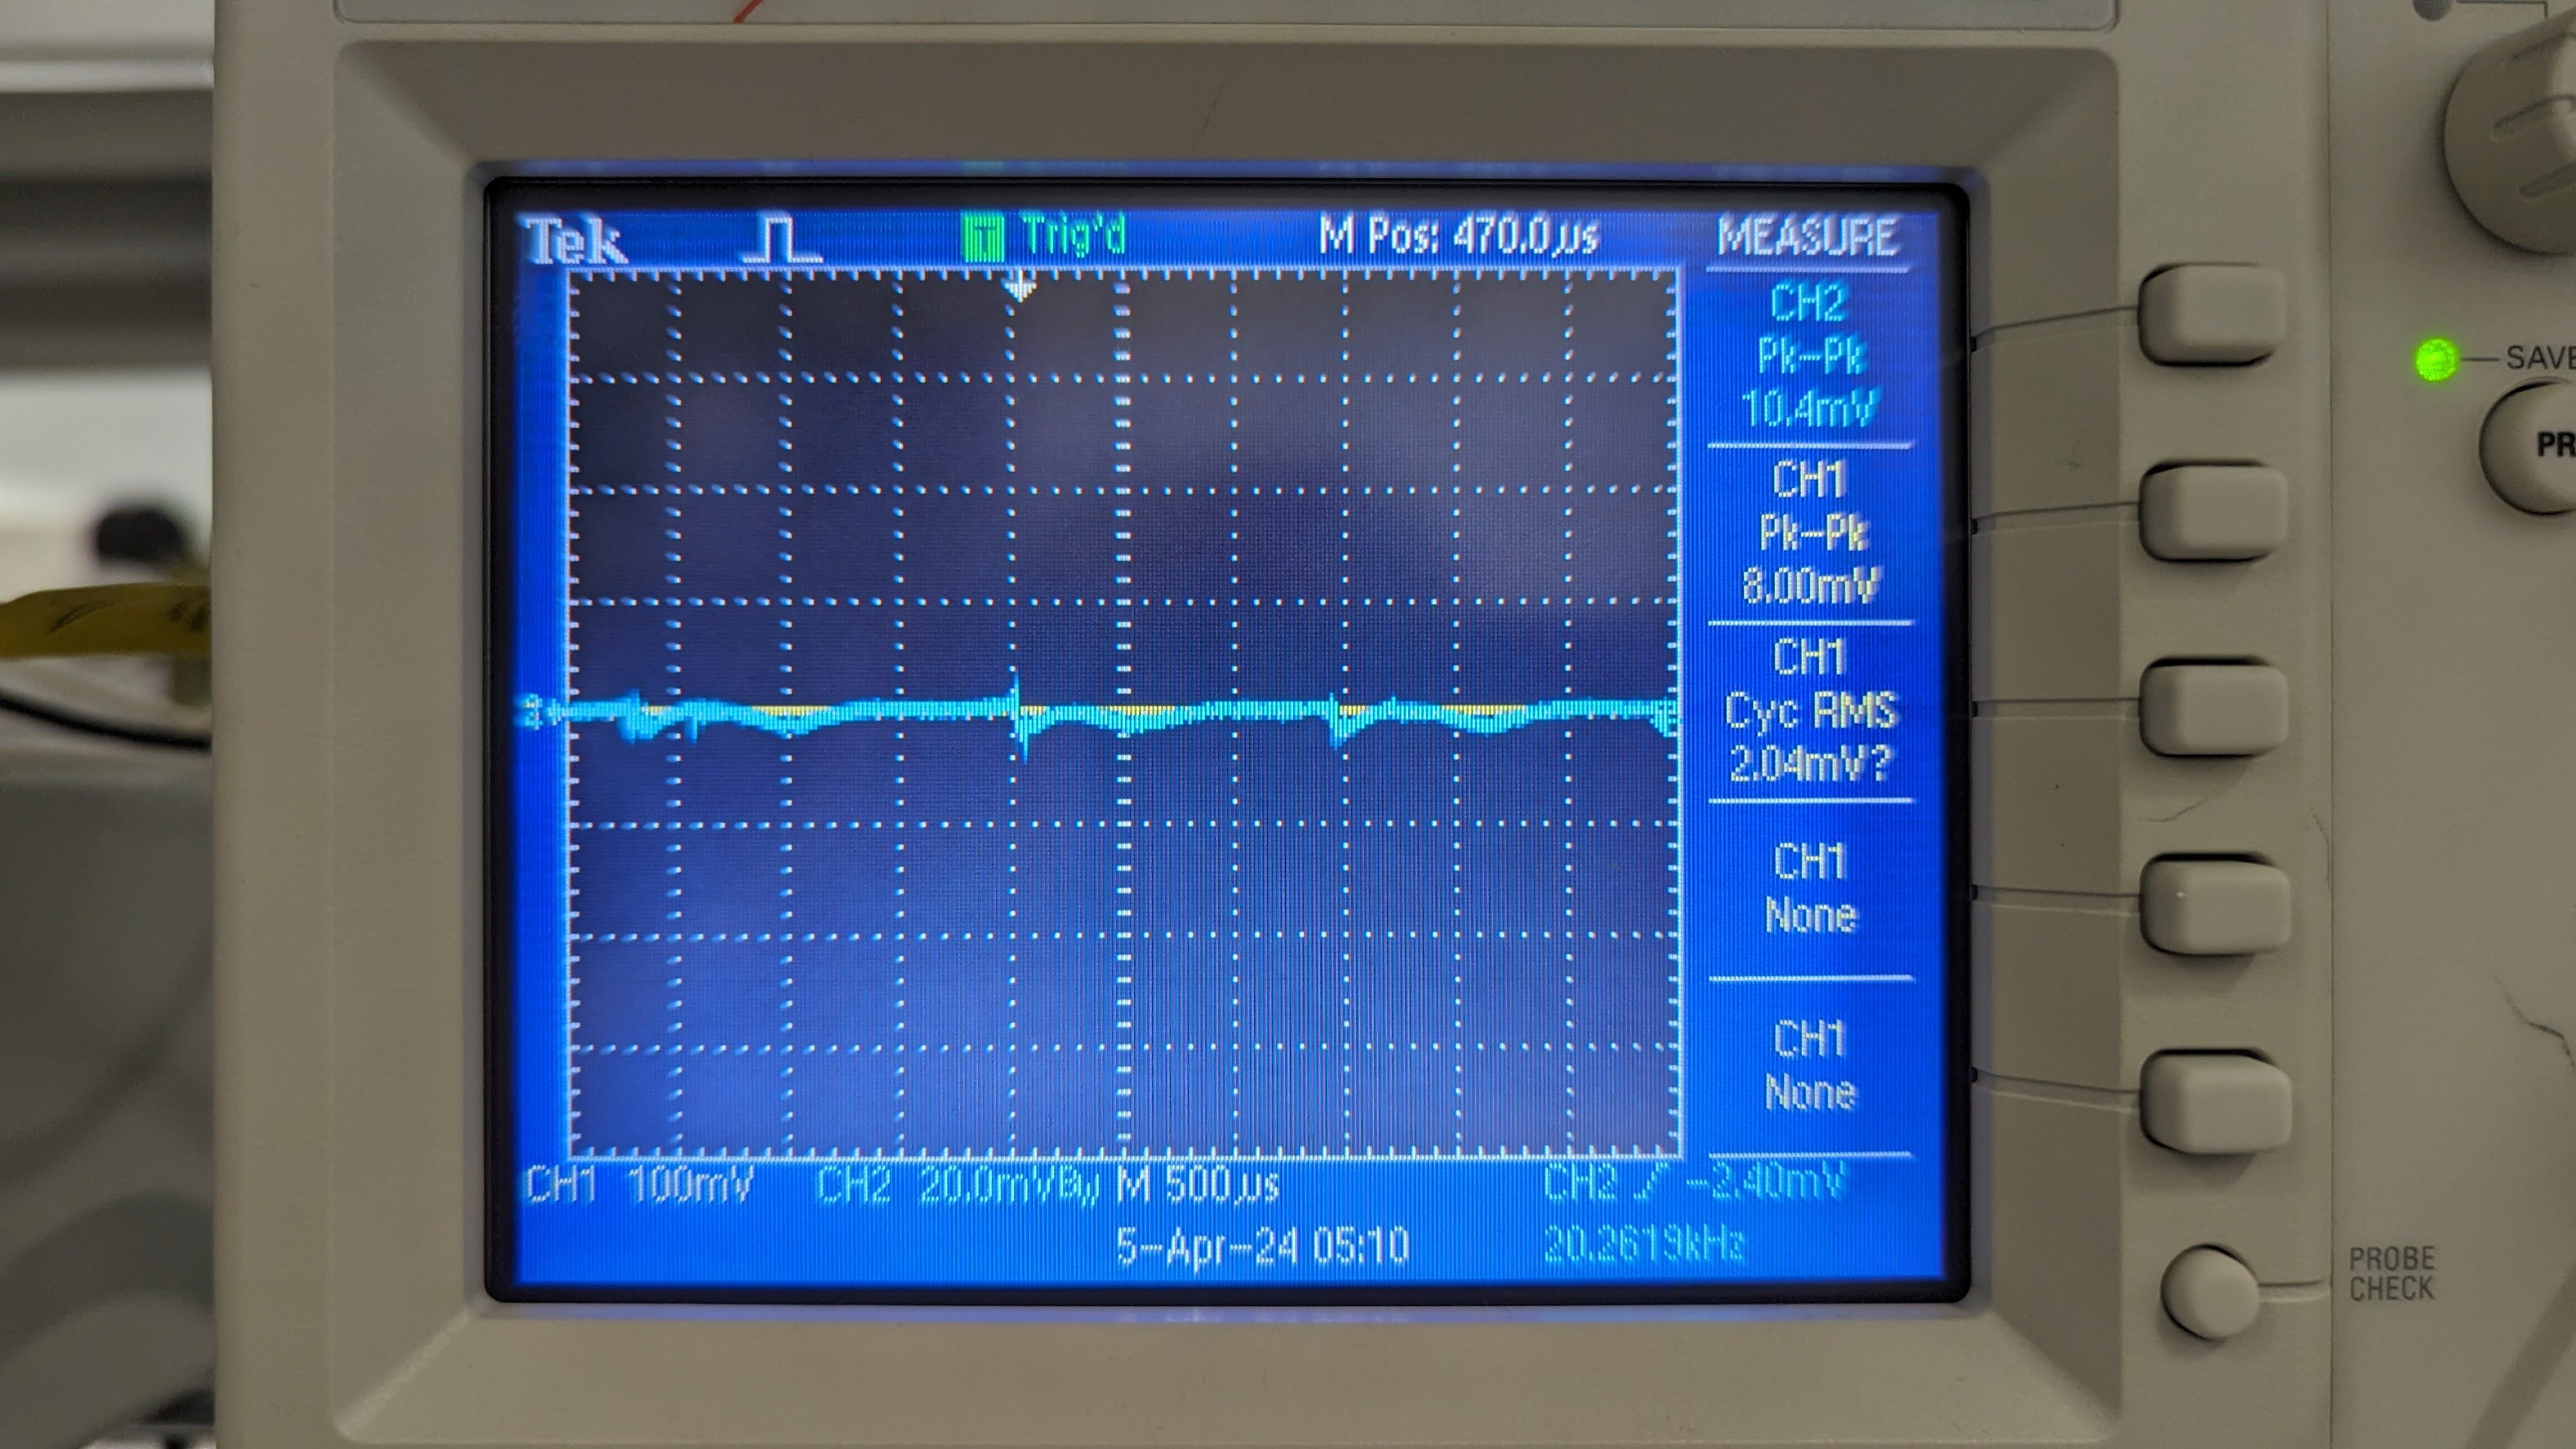
\includegraphics[width=0.7\textwidth]{q2-5}
    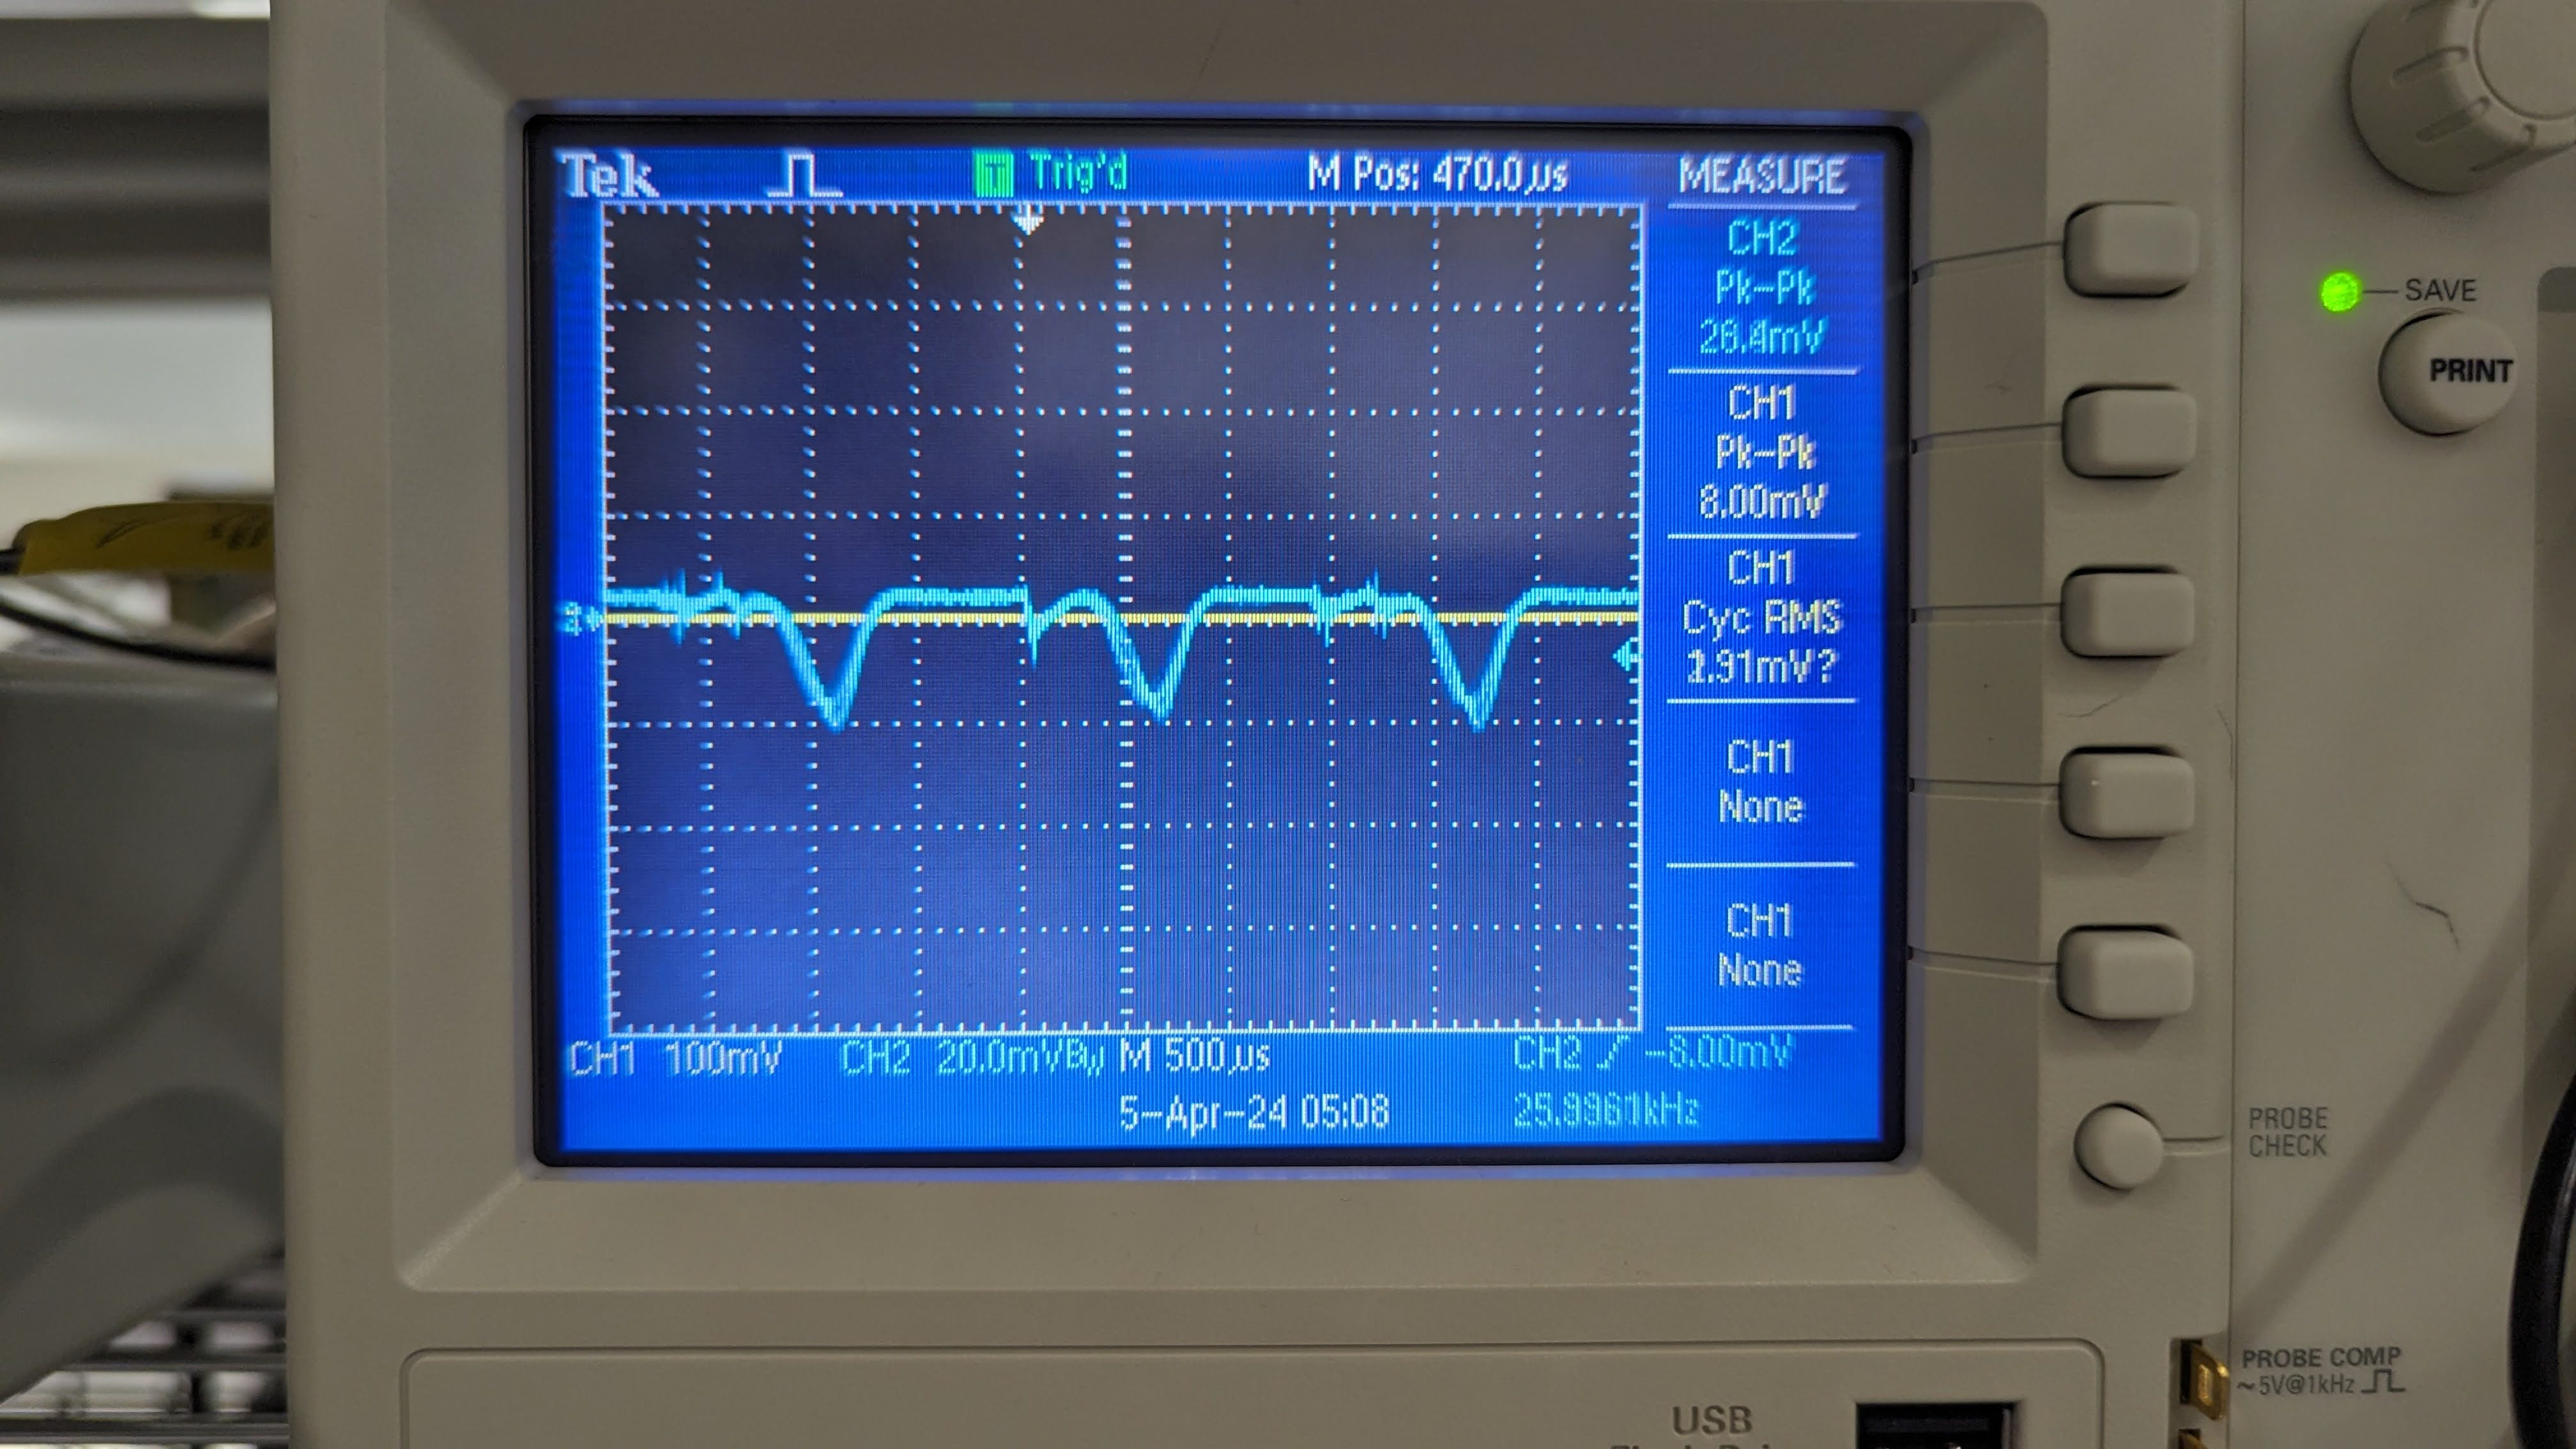
\includegraphics[width=0.7\textwidth]{q2-2}
    \caption{Waveforms for Task 2 part 2. Left is for 5mm, while right is 2mm. Scopes are maximally zoomed in, but the signal is still extremely small. In case the graphs turn out unreadable on print, the only relevant text is the left reading is Pk-Pk 10.4mV and the right is 26.4mV.}
    \label{fig:q2}
\end{figure}


{\medskip\noindent\bf Question 3.} For 5mm, we measured the peak voltage of the amplified signal to be 960mV using an oscilloscope. Similarly for $2$mm we found it to be 1.9V, although again both these numbers are quite sensitive to the exact distance of the wheel which wasn't very repeatable. We measured the voltage across the $R_C$ resistor of Q3 to be $4.7$ both for 2mm and 5mm, so $I_{C,3}=\frac{4.7}{3900}=1.2$mA. For the gain, comparing these values to those in part 2 for the 5mm case, we get a gain of $A_v= \frac{960}{10.4}=92.3$.

For the small signal analysis, note that the circuit on the left side is the exact same one studied in class and during the previous lab. The small signal equivalent can be seen in figure \ref{fig:q3}. For this circuit we found $g_m= \frac{I_C}{V_T}=\frac{1.2\cdot 10^{-3}}{0.025}=0.048$A/V. Using this (and our value of $\beta$ from lab 3) we find that
\[
    r_{\pi}=\frac{\beta}{g_{m}}=3.46k\Omega\implies R_{in}= R_1 // R_2 / / r_{\pi}=2.96k\Omega
\]
\[
\implies A_v=-g_m \left( \frac{R_{in}}{R_S+R_{in}} \right) \left( R_C / / R_L \right) =130.4
.\]

There is a large discrepancy between our experimental gain (92.3) and the theoretical (130.4). One explanation is that the small voltage we read during part 2 was before the signal was amplified and thus at very low resolution for the oscilloscope we were using. The wheel was also moved between the two measurements and the positioning for 5mm was difficult to get consistent, so this also contributed to a different source signal between the two measurements. Finally the BJT we used was not the exact same one we calculated the gain for in the previous lab, so there could have been a component-specific difference that led to the discrepancy.

\begin{figure}[htpb]
    \centering
    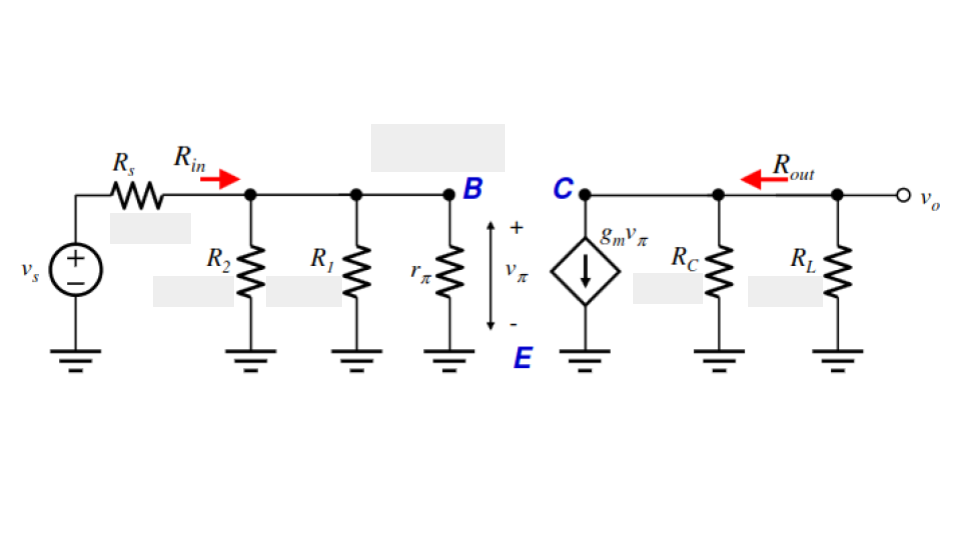
\includegraphics[width=0.8\textwidth]{q3}
    \caption{Small circuit equivalent for task 2 part 3. This diagram was adapted from the lecture slides, since the circuit is functionally identical to there. Here $R_1=56k\Omega$, $R_2=33k\Omega$, $R_C=3.9k\Omega$, $R_L=100k\Omega$. From the Hall effect sensor's datasheet, we have that $R_s=1140\Omega$.}
    \label{fig:q3}
\end{figure}

{\medskip\noindent\bf Question 4.} When adjusted from 5mm to 2mm, the rectified voltage went from 0.7V to 1.2V. There was no visible ripple (other than non-periodic noise on the order of 100mV), although since for this part we disconnected the load (the motor driver) this is expected as there's no current draw from the capacitor. We found peak voltages of 0.96V and 1.9V in the previous part for 5mm and 2mm respectively. Thus the diode drop for 2mm is 1.9-1.2=0.7V as expected, although for 5mm the drop of 0.96-0.7=0.26V is definitely lower than expected. This might just have to do with the positioning of the wheel though, as especially for 5mm it was difficult to get a consistent placement of the wheel.

Interestingly, after going from 5mm to 2mm and seeing the voltage vary, when bringing it back from 2mm to 5mm the voltage barely changed. Initially this was confusing to us, but since there's no load on the capacitor (and it can't discharge through the diode of course) it stays charged even when the rectified voltage is too low to charge it anymore.

{\medskip\noindent\bf Question 5.} At 5mm, we saw 270mV at the base of Q1, and as we gradually moved to 2mm it changed to 640mV. As for qualitative changes, the further the motor was away from the magnets the faster it spun. Thus the motor controller varies the speed of the motor inversely proportional to the distance from the sensor.

The mechanism of the motor control is a few stages. The first is the Hall effect sensor, which converts the rotary motion into a small signal whose magnitude represents how close the sensor is to the motor. Next a BJT amplifier is used to make this signal larger, and it is rectified to a DC voltage using a diode and a capacitor at a. Next the inverter investigated at the beginning of this lab inverts this signal, and finally it is fed into the DC motor to vary the motor speed opposite to the distance from the sensor.

\end{document}
